\begin{figure}[htb]
    \centering
         \begin{tikzpicture}
            \begin{axis}[
                xlabel={$t / ms$},
                ylabel={$i'/ i'* / A$},
                axis lines=left,
                ymin=0, ymax=30,
                xmin=0, xmax=10,
                xtick={0,1,2,3,4,5,6,7,8,9,10},
                ytick={0,5,10,15,20,25,30},
                thick,
                smooth,
                no markers,
                height=7cm,
                width = 0.99\textwidth,
                grid
                ]
                % Plot adjusted quadratic function
                \addplot[signalblue, domain=0:10, samples=200] {24.5 * (1 - ((x-5)/5)^2)};
                
            \addplot[
                thick,
                mark=none,
                color=black,
            ] coordinates {
                (1.25,8.6)  (1.4,12.2)             (1.532,5.5)    (1.855,16.4) 
                (2.058,8.3) (2.31,19.9)           (2.55,11.3)    (2.765,22.7)  
                (3.15,14.5)  (3.3,24.9)          (3.65,17.2)    (3.8,26.3)
                (4.15,19.5)   (4.3,27.2)           (4.65,21)   (4.75,27.8)
                (5.2,21.8)   (5.3,27.9)         (5.65,21.5)   (5.75,27.5)
                (6.15,20.5)   (6.25,26.9)         (6.7,18.7)   (6.8,25.8)
                (7.1,16.3)   (7.3,24.2)         (7.6,13.5)   (7.75,21.9)
                (8.1,10.5)   (8.3,19)         (8.6,7.5)    (8.8,15.1)
                (9,4.5)     (9.4,10.2)         (9.5,1.8)   (9.9,4.2)
                (10,0)
            };
            \end{axis}
        \end{tikzpicture} 
        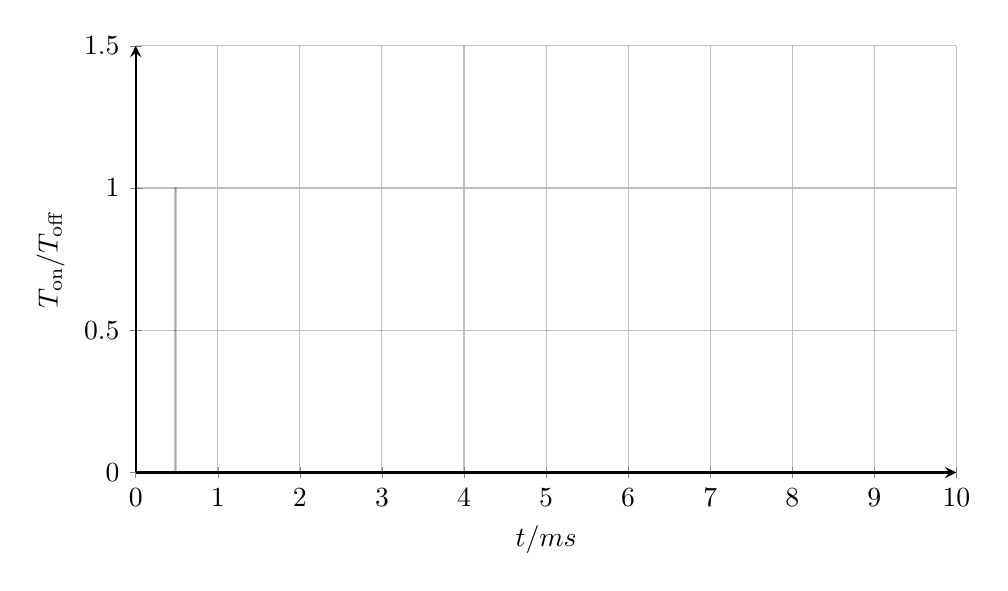
\begin{tikzpicture}
            \begin{axis}[
                xlabel={$t / ms$},
                ylabel={$T_\mathrm{on}/T_\mathrm{off}$},
                axis lines=left,
                ymin=0, ymax=1.5,
                xmin=0, xmax=10,
                xtick={0,1,2,3,4,5,6,7,8,9,10},
                ytick={0,0.5,1,1.5},
                thick,
                smooth,
                height=7cm,
                width=0.99\textwidth,
                grid
                ]
                % Draw rectangle
                \draw[fill=black, opacity=0.2] (axis cs:0.48, 0) rectangle (axis cs:0.49, 1);
            \end{axis}
        \end{tikzpicture}
    \caption{TEST}
    \label{fig:QuadraticFunction}
\end{figure}
